\chapter{IMPLEMENTATION DETAILS}
\vspace{0.5in}
\begin{figure}[h]
    \centering
    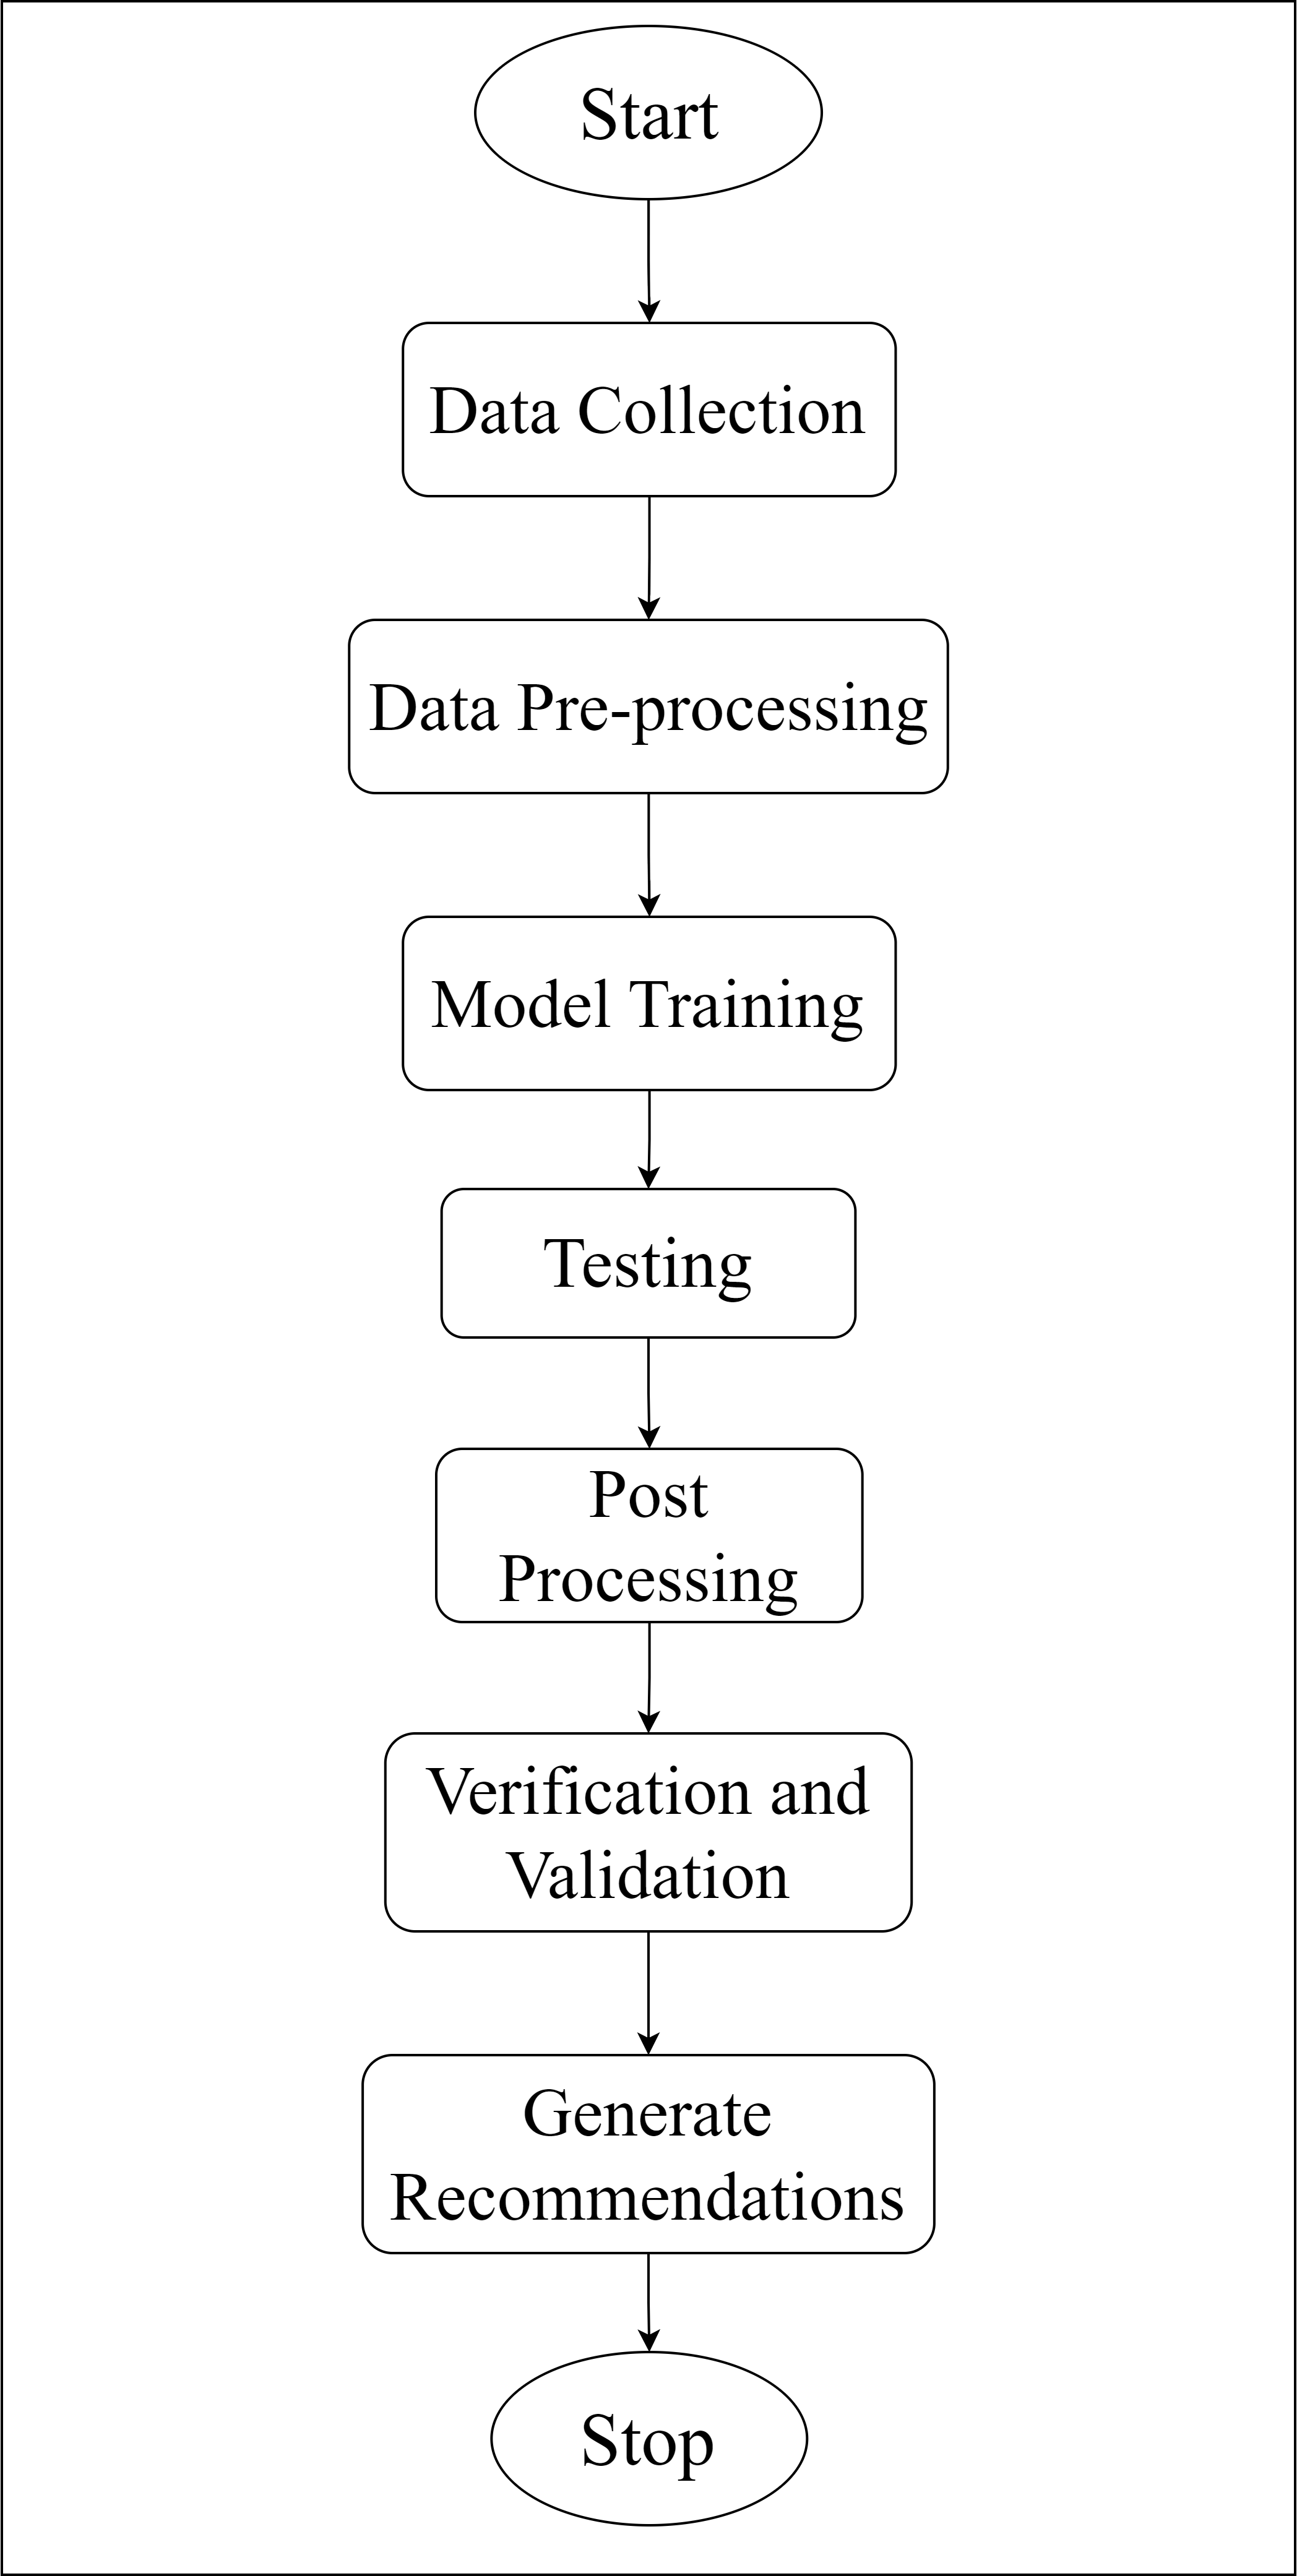
\includegraphics[width=0.6\linewidth]{img/Graphics/System_flow_BRS.drawio.png}
    \caption{System Flowchart}
    \label{Flowchart}
\end{figure}

Throughout the course of this project, Comparative Analysis of Recommendation Systems to recommend books, various machine learning models have been implemented, trained and tested in order to provide best possible resultant recommendation for users. In order to effectively execute the project objectives alongside a well maintained large database, the fine tuning of various models is essential. The major steps involved in this project are as listed below :
\begin{itemize}
    \item Dataset Collection
    \item Pre-processing the data
    \item Model Training
    \item Testing
    \item Post Processing
    \item Verification and Validation
\end{itemize}

\subsection{Dataset Collection}
The dataset is collected from Kaggle. This dataset comprising of three tables for users, books and ratings was compiled by Cai-Nicolas Ziegler. The dataset was formed on the basis of books read by users and ratings provided by them on Amazon and the online data for books from Amazon along with user ratings and users who bought them. The dataset was originally in .CSV format.

\subsection{Pre-processing the data}
Data Preprocessing is the most crucial part before training the model.
It involves cleaning and transforming the raw data into a format which is suitable for analysis or training machine learning models. Data preprocessing is essential because raw data often contains noise, inconsistencies, and missing values that can negatively impact the performance of machine learning models. A well-preprocessed dataset can lead to better model training and reliable analysis.

     After the dataset has been loaded into the system, the next step in machine learning pipeline is data preprocessing. The data has been inspected to check for inconsistencies, duplicate values and missing values. The missing values in the dataset were replaced by the mode value of respective column. The mode was chosen as viable alternative amongst choices of removing entire row or by replacing with mean, median of interpolated values.
     Further cleaning the data involved removing books that have less than 50 total reviews,
         removing ratings from users who have less than 200 reviews to maintain statistical relevancy and
         finding all duplicates with different ISBN, deleting the extras and updating the ones to keep. For this, all the books with the same title and author were found and the ratings were updated to point to the 1st ISBN found for that book. This helped reduce sparsity in the user-item interaction matrix and focuses on more active users and items. 
     Extreme ratings that could skew the results (outliers) are risky but they were retained since they are relevant for the recommendation model.

\subsection{ Model Training}

After data pre-processing the next step in Machine Learning pipeline is Model Training. Here, in this project we have trained four different models 
\begin{itemize}
    \item KNN
    \item Matrix Factorization
    \item Dense Neural Network
    \item Jaccard's Similarity
\end{itemize}

Since the training procedures of each of the following models are different the next this step in our project forks out into diffrent branches.For each of the model training, testing and implementation we have used Google Collaboratory as working platform utilizing the GPU resource it provides.

\subsection*{KNN}
k-Nearest Neighbors (KNN) is a type of supervised learning algorithm used for regression tasks which predicts the label or value of a data point based on the average of its k-nearest neighbors in the feature space.
Here for implementation of KNN we have utilized 'NearestNeighbours' class of scikit-learn library, which enables to find the k-neighbours for given book in feature space \\
\textbf{Choice of Hyperparameter k:} k represents the number of neighbors considered for each prediction. The fine tuning of hyperparameter is very essential as smaller too small k can lead to overfitting, while too large k can result in underfitting.
After iterative testing the value of k was choosen to be 7.

\subsection*{Matrix Factorization}
Matrix Factorization is a collaborative filtering technique commonly used in book recommendation systems. It involves decomposing the user-item interaction matrix into two lower-dimensional matrices representing users and items with the aim that when reconstructed back again it captures hidden pattern or the latent factors that help to predict missing values and generate personalized recommendations.
For the implemendation and training of Matrix Factorization first of all a sparse matrix of user-item i.e UserID-BookId was formed which is also commonly known as pivot column. Then the 'TruncatedSVD' class was used to perform dimensionality reduction on the transpose of this pivot column which was then fitted into Matrix Factorization model whose resultant would provide recommendations.

\subsection*{Neural Network}
A Neural Network is a machine learning model inspired by the structure and functioning of the human brain. It consists of layers of interconnected nodes, or neurons, organized into an architecture that allows the model to learn patterns and relationships in data. Dense layers, also known as fully connected layers, are a type of layer in a neural network where each neuron is connected to every neuron in the previous and subsequent layers. These layers are often used to capture complex patterns and relationships in the data. Optimization techniques are algorithms used to adjust the model's parameters during training in order to minimize the error or loss. Adam optimizer has been used which is a  popular optimization algorithm that combines the benefits of both the AdaGrad and RMSProp algorithms. Mean Squared Error (MSE) has been used as the loss function. The optimizer is responsible for updating the model's weights during training, while the loss function quantifies how well the model is performing by measuring the difference between the predicted values and the actual values. The model was trained for a total of 50 epochs. 

\begin{figure}[h]
    \centering
    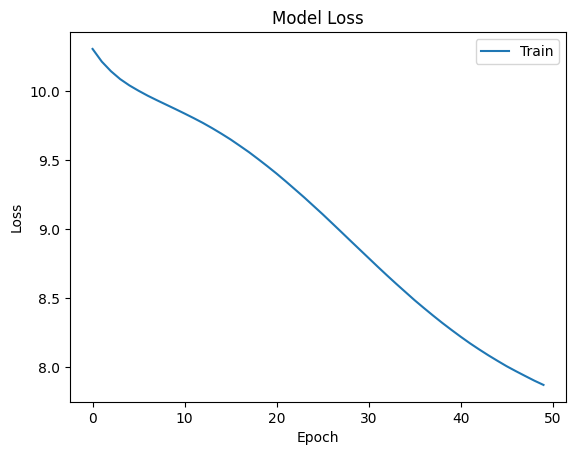
\includegraphics[width=1\linewidth]{img/Graphics/loss-in-nn.png}
    \caption{Loss Per Epoch}
    \label{loss-in-nn}
\end{figure}
\newpage

The figure \ref{loss-in-nn} shows the value of the loss function that the model experienced during the training process. Mean Squared Error(MSE) is the loss function. The curve above shows the value of the loss function during training per epoch. The term "loss" refers to a measure of how well a model's predictions match the true labels or target values in the training data. It can be seen that the loss function takes a value that is above 10 during the beginning of the training process. The loss per epoch goes on continuously decreasing with every epoch and reduces to below 8 by the end of the training process.


\subsubsection*{ Jaccard's Similarity}
Jaccard's Similarity is the measusre of similarity between two sets. A user-item interaction matrix has been constructed where rows represent users and columns represent books and the entries in the matrix represent user interactions or ratings. A user-user similarity matrix has also been constructed based on the similarity between users. Jaccard's Similarity has been used to measure this similarity. The Jaccard's Similarity between two users is calculated based on their interactions with items. It measures the similarity in terms of the items they have interacted with via the rating values. The formula for Jaccard's Similarity is applied to the sets of items each user has interacted with. It computes the ratio of the number of common items to the total number of unique items across both users. Once the user-user similarity matrix had been constructed using Jaccard's Similarity or other similarity measures, it provided a numerical representation of how similar each pair of users is. To generate recommendations for a target user, the system identifies users who are most similar to the target user based on the user-user similarity matrix. Items liked or interacted with by similar users but not by the target user were then recommended to the target user. This assumes that users with similar preferences will likely appreciate items that the target user has not yet interacted with.


\subsection{Post Processing}
The proposed models have generated top recommendations based on the top ratings. The books were sorted on the basis of their ratings in descending order and the top books were extracted. Similarly each model generated suitable recommendations based on the training done upon them and the context provided i.e. name of the book.

\subsubsection*{Similarity metric}
   In the context of a book recommendation system using user-item interactions, cosine similarity has been used to measure the similarity between vectors representing books based on user rating.
        Euclidean distance has been used to calculate the distance between the user ratings. The smaller the distance, the more similar the books are.

\par
The model has been trained by feeding the cleaned data into the model based on which the model has predicted the values. The predicted values have been compared with actual values from google and amazon recommendation engine to gain insight into the models' performance. The precision, recall and f1-score of our system has been calculated. The hyper-parameter has tuned using the cross validation technique.

\newpage

\subsection{Verification and Validation}
Precision reflects the models ability to avoid recommending irrelevant items. A good precision rate indicates that when the model recommends items, they are more likely to be liked by the user.
\begin{equation}
\label{precision}
      Precision = \frac{True Positives}{True Positives + False Positives}
\end{equation}
Recall suggests how effective the model is at recommending the relevant elements. For almost all recommendation systems, higher recall is more important than higher precision as capturing as many relevant items as possible is the highest priority for these type of system.
\begin{equation}
\label{recall}
      Recall = \frac{True Positives}{True Positives + False Negatives} 
\end{equation}
F1-score is particularly useful when there is a need to balance precision and recall. It takes into consideration both false positives and the false negatives, giving a more comprehensive evaluation of the model's performance.
\begin{equation}
    \label{f1-score}
          F1-score = \frac{2*Precision*Recall}{Precision + recall} 
\end{equation}
where, \\
True Positives = Items that were correctly recommended and were actually liked by the user. \\
False Positives = Items that were recommended but were not liked by the user.

\vspace{4mm}
\begin{table}[h]
    \centering
    \caption{Model Comparison with respect to the Recommendations of Google \& Amazon}
    \begin{tabular}{|p{0.8in}|p{0.8in}|p{0.8in}|p{0.8in}|}
\hline
        Metrics & kNN & MF & JS \\
        \hline
        Precision & 0.3294 & 0.2972 & 0.3101\\
        Recall & 0.5944 & 0.5544 & 0.6185\\
        F1-Score & 0.3959 & 0.3743 & 0.4005\\
        \hline
    \end{tabular}
    \vspace{2 mm}
    \label{Model Comparison}
\end{table}

\begin{table}[h]
    \centering
    \caption{Averaged Metrics after Comparing the Models to each other}
    \begin{tabular}{|p{0.8in}|p{0.8in}|p{0.8in}|p{0.8in}|p{0.8in}|}
\hline
        Metrics & kNN & MF & JS & NN \\
        \hline
        Precision & 0.8045 & 0.5429& 0.6645 & 0.5745 \\
        Recall & 0.7503 & 0.9595& 0.7528 & 0.8601 \\
        F1-Score & 0.7410 & 0.6825& 0.6264 & 0.6889 \\
        \hline
    \end{tabular}
    \vspace{2 mm}
    \label{Model Comparison-2}
\end{table}

\newpage
\section{Dataset Explanation}
The well-maintained and well-documented dataset for Book recommendation system has been acquired from Kaggle. The 'Book-recommendation' dataset that we're currently using has been mined by Cai-Nicolas Ziegler. The 'Book-recommendation' dataset is comprised of 3 files. 
    \subsection{Books} 
    Books are identified by unique ISBN numbers. The content-based information of books comprises of labelled data under headings  Book-Title, Book-Author, Year-Of-Publication and Publisher.
    When there are multiple authors, just the first one is listed. Additionally, three distinct attributes  Image-URL-S, Image-URL-M, and Image-URL-L, or small, medium, and big, are provided for the URLs that link to the cover images. These web addresses lead to the Amazon website.\\
   \begin{figure}[h]
       \centering
       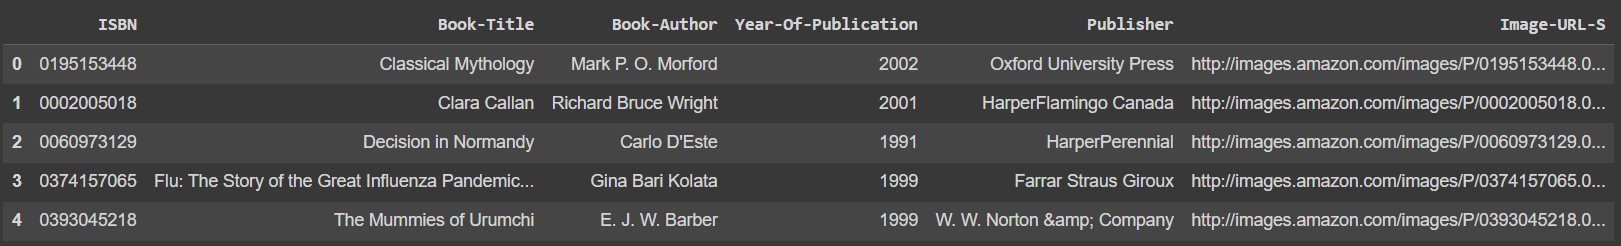
\includegraphics[width=150mm]{img/Graphics/books.png}
       \caption{Simplified Dataset prototype Books}
       \label{fig:enter-label}
   \end{figure}
  
    \subsection{Users}
    In the User-dataset, User-ID have been anonymized and mapped to integers. Additionally demographic data based on Location, Age(if available) is provided. This is particularly necessary for collaborative based filtering. This data table is further merged with the book dataset for further analysis and evaluation of the various ml models.\\

    \begin{table}[h]
    \centering
    \caption{Simplified Dataset prototype: Users}
    \begin{tabular}{|p{0.2in}|p{0.6in}|p{0.9in}|p{0.8in}|}
\hline
         & User-ID & Location & Age \\
        \hline
        0 & 1 & nyc, new york, usa & 19.0 \\
        1 & 2 & stockton, california, usa & 18.0\\
        \hline
    \end{tabular}
    \vspace{2 mm}
    
    \label{Simplified Dataset prototype: Users}
\end{table}

    
    \subsection{Ratings} 
    Book-Ratings are explicit, expressed on a scale from 1-10 (higher values implies higher appreciation), or implicit, expressed by 0. There contains foreign keys such as User-ID and ISBN which connects this table with other tables for data visualization and data for frontend UI.\\
     \begin{table}[h]
    \centering
    \caption{Simplified Dataset prototype: Ratings}
    \begin{tabular}{|p{0.2in}|p{0.6in}|p{0.9in}|p{0.8in}|}
\hline
         & User-ID & ISBN & Book-Rating \\
        \hline
        0 & 276725 & 034545104X & 5 \\
        1 & 276726 & 0155061224 & 9\\
        \hline
    \end{tabular}
    \vspace{2 mm}
    
    \label{Simplified Dataset prototype: Ratings}
\end{table}
\newpage